\section{Trading System Design}

%\begin{figure}[H]
%\centerline{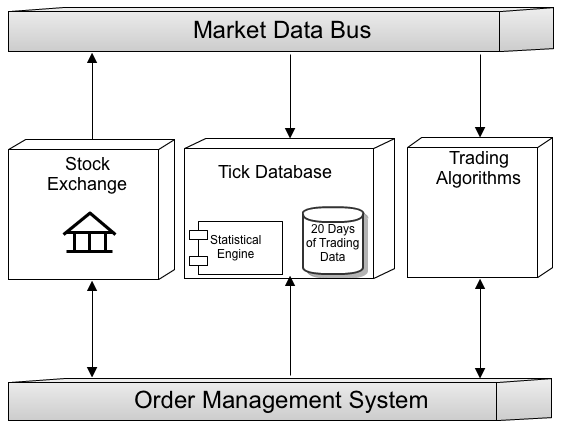
\includegraphics[scale=0.6]{trading-system-design.png}}
%\caption{Trading System Architecture}
%\label{fig:trading-system-architecture}
%\end{figure}

\subsection{Stock Exchange}
Market Participants submit orders to the Stock Exchange in order to trade. Stock Exchanges publish messages about the submitted/executed orders.

\subsection{Market Data Bus}
Market Data Bus subscribes to messages published by different Stock Exchanges in order to publish them in a standardised way to various internal systems, e.g. Trading Algorithms.

\subsection{Order Management System}
Registers with various Stock Exchanges in order to provide a standardised way of submitting orders by various internal systems, e.g. Trading Algorithms, and also allow Automatic Order Routing between different Stock Exchanges.

\subsection{Tick Database}
Subscribes to the Market Data Bus in order to perform a statistical analysis on the behaviour of different stocks. The result of the statistical analysis is a set of parameters which describe various aspects of stock behaviour. The parameters are published to various internal systems, e.g. Trading Algorithms.

\subsection{Trading Algorithms}
Highly sophisticated and parameterised systems which accept orders and execute them using different strategies. Trading Algorithms register with the Market Data Bus in order to react to the current situation on the market. They continuously compare the behaviour of stocks with their historical behaviour (using data from the Tick Database) in order to quickly discover unexpected behaviour. 
